\documentclass{article}

\usepackage[papersize={30cm,21cm},left=0cm,right=0cm,top=0cm,bottom=0cm]{geometry}
\usepackage{tikz}              % zum Zeichnen von Abbildungen etc.
\usetikzlibrary{backgrounds,mindmap}

\definecolor{f1}{HTML}{7FA0A0}
\definecolor{f2}{HTML}{1133FF}
\definecolor{f3}{HTML}{36648B}
\definecolor{f7}{HTML}{5692B4}
\definecolor{f5}{HTML}{78BCEE}
\definecolor{f6}{HTML}{00FFFF}
\definecolor{f9}{HTML}{00DD99}
\definecolor{f8}{HTML}{FFFFA6}
\definecolor{f4}{HTML}{00CC66}
\definecolor{f10}{HTML}{00BB22}
\definecolor{darkgreen}{HTML}{006600}
\definecolor{scipyellow}{HTML}{FFFFE6}

\pagestyle{empty}

\begin{document}

\centering
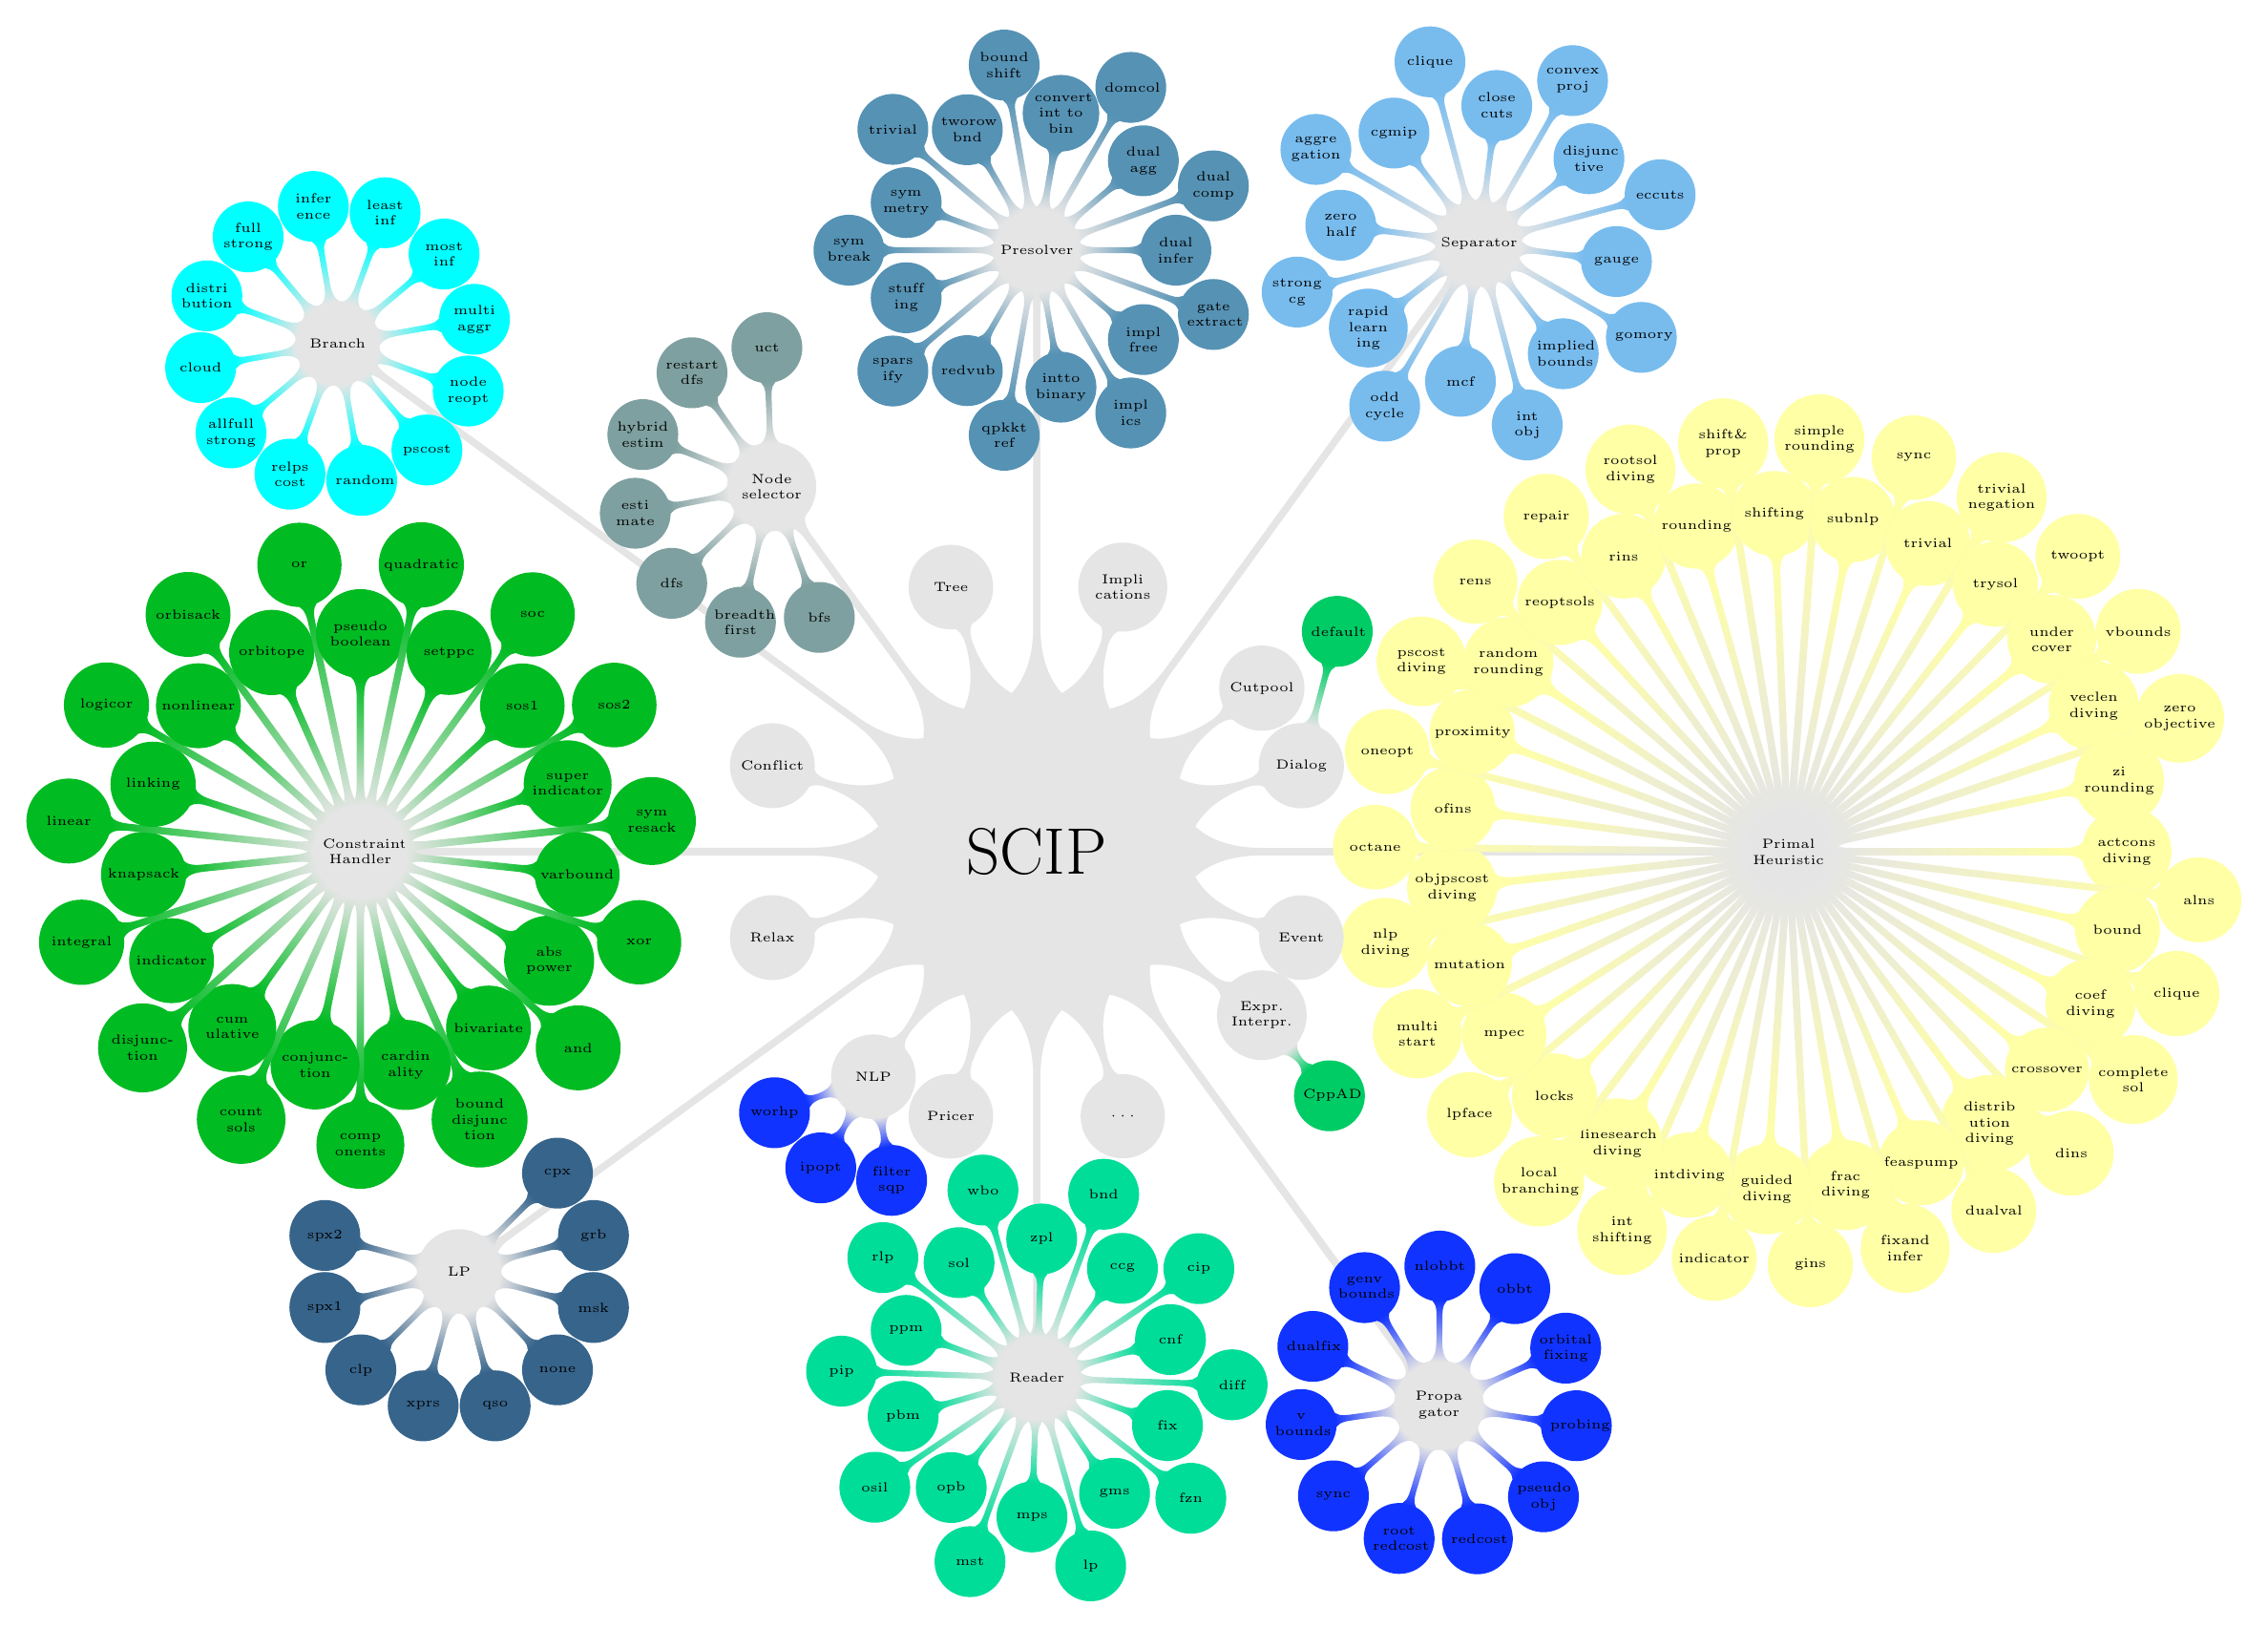
\begin{tikzpicture}[mindmap,concept color=gray!20]
  \tikzstyle{root concept} = [concept, text width=1cm, minimum size=1cm, sibling angle=18];
  \tikzstyle{level 1 concept} = [level 3 concept,level distance=3.7cm,sibling angle=18, minimum size=.7cm];
  \tikzstyle{level 2 concept} = [level 4 concept];%sibling angle=18, minimum size=1cm, text width=1cm];
  \tikzstyle{branchconcept} = [level 2 concept,concept color=f6];
  \tikzstyle{conshdlrconcept} = [level 1 concept,sibling angle=25,concept color=f10,minimum size=.6cm];
  \tikzstyle{conshdlrconceptodd} = [conshdlrconcept, sibling angle=12, level distance=3.9cm];
  \tikzstyle{conshdlrconcepteven} = [conshdlrconceptodd, level distance=2.9cm];
  \tikzstyle{lpiconcept} = [level 2 concept,concept color=f3];
  \tikzstyle{dialogconcept} = [level 2 concept,concept color=f4];
  \tikzstyle{displayconcept} = [level 2 concept,concept color=f4];
  \tikzstyle{nodeselectionconcept} = [level 2 concept,sibling angle=33,concept color=f1];
  \tikzstyle{presolverconceptodd} = [level 2 concept,sibling angle=20,concept color=f7];
  \tikzstyle{presolverconcepteven} = [presolverconceptodd, level distance=2.5cm];
  \tikzstyle{heurconceptodd} = [level 1 concept, sibling angle=6.69, level distance=5.5cm, concept color=f8, minimum size=.7cm];
  \tikzstyle{heurconcepteven} = [heurconceptodd, level distance=4.5cm, minimum size=.7cm];
  \tikzstyle{readerconceptodd} = [level 2 concept,sibling angle=18,concept color=f9];
  \tikzstyle{readerconcepteven} = [readerconceptodd, level distance=2.6cm];
  \tikzstyle{sepaconceptodd} = [level 2 concept,sibling angle=22.5,concept color=f5];
  \tikzstyle{sepaconcepteven} = [sepaconceptodd,level distance=2.5cm];
  \tikzstyle{propconcept} = [level 2 concept,sibling angle=32.7,concept color=f2];
  \tikzstyle{eventconcept} = [level 2 concept,concept color=f4];
  \tikzstyle{nlpiconcept} = [level 2 concept, level distance=1.4cm,sibling angle=40,concept color=f2];
  \tikzstyle{exprintconcept} = [level 2 concept, level distance=1.4cm,concept color=f4];

  \node [concept] {\Huge SCIP}
  [clockwise from=0]
  child[level distance=10cm] { node[concept] (Heuristic) {Primal\\Heuristic}
	child[heurconcepteven] { node[concept] (actconsdiving) {actcons\\diving}}
	child[heurconceptodd] { node[concept] (alns) {alns}}
	child[heurconcepteven] { node[concept] (bound) {bound}}
	child[heurconceptodd] { node[concept] (clique) {clique}}
	child[heurconcepteven] { node[concept] (coefdiving) {coef\\diving}}
	child[heurconceptodd] { node[concept] (completesol) {complete\\sol}}
	child[heurconcepteven] { node[concept] (crossover) {crossover}}
	child[heurconceptodd] { node[concept] (dins) {dins}}
	child[heurconcepteven] { node[concept] (distributiondiving) {distrib\\ution\\diving}}
	child[heurconceptodd] { node[concept] (dualval) {dualval}}
	child[heurconcepteven] { node[concept] (feaspump) {feaspump}}
	child[heurconceptodd] { node[concept] (fixandinfer) {fixand\\infer}}
	child[heurconcepteven] { node[concept] (fracdiving) {frac\\diving}}
	child[heurconceptodd] { node[concept] (gins) {gins}}
	child[heurconcepteven] { node[concept] (guideddiving) {guided\\diving}}
	child[heurconceptodd] { node[concept] (indicator) {indicator}}
	child[heurconcepteven] { node[concept] (intdiving) {intdiving}}
	child[heurconceptodd] { node[concept] (intshifting) {int\\shifting}}
	child[heurconcepteven] { node[concept] (linesearchdiving) {linesearch\\diving}}
	child[heurconceptodd] { node[concept] (localbranching) {local\\branching}}
	child[heurconcepteven] { node[concept] (locks) {locks}}
	child[heurconceptodd] { node[concept] (lpface) {lpface}}
	child[heurconcepteven] { node[concept] (mpec) {mpec}}
	child[heurconceptodd] { node[concept] (multistart) {multi\\start}}
	child[heurconcepteven] { node[concept] (mutation) {mutation}}
	child[heurconceptodd] { node[concept] (nlpdiving) {nlp\\diving}}
	child[heurconcepteven] { node[concept] (objpscostdiving) {objpscost\\diving}}
	child[heurconceptodd] { node[concept] (octane) {octane}}
	child[heurconcepteven] { node[concept] (ofins) {ofins}}
	child[heurconceptodd] { node[concept] (oneopt) {oneopt}}
	child[heurconcepteven] { node[concept] (proximity) {proximity}}
	child[heurconceptodd] { node[concept] (pscostdiving) {pscost\\diving}}
	child[heurconcepteven] { node[concept] (randrounding) {random\\rounding}}
	child[heurconceptodd] { node[concept] (rens) {rens}}
	child[heurconcepteven] { node[concept] (reoptsols) {reoptsols}}
	child[heurconceptodd] { node[concept] (repair) {repair}}
	child[heurconcepteven] { node[concept] (rins) {rins}}
	child[heurconceptodd] { node[concept] (rootsoldiving) {rootsol\\diving}}
	child[heurconcepteven] { node[concept] (rounding) {rounding}}
	child[heurconceptodd] { node[concept] (shiftandpropagate) {shift\&\\prop}}
	child[heurconcepteven] { node[concept] (shifting) {shifting}}
	child[heurconceptodd] { node[concept] (simplerounding) {simple\\rounding}}
	child[heurconcepteven] { node[concept] (subnlp) {subnlp}}
	child[heurconceptodd] { node[concept] (sync) {sync}}
	child[heurconcepteven] { node[concept] (trivial) {trivial}}
	child[heurconceptodd] { node[concept] (trivialnegation) {trivial\\negation}}
	child[heurconcepteven] { node[concept] (trysol) {trysol}}
	child[heurconceptodd] { node[concept] (twoopt) {twoopt}}
	child[heurconcepteven] { node[concept] (undercover) {under\\cover}}
	child[heurconceptodd] { node[concept] (vbounds) {vbounds}}
	child[heurconcepteven] { node[concept] (veclendiving) {veclen\\diving}}
	child[heurconceptodd] { node[concept] (zeroobj) {zero\\objective}}
	child[heurconcepteven] { node[concept] (zirounding) {zi\\rounding}}
  }
%   child { node[concept] (Variable) {Variable}}
  child { node[concept] (Event) {Event}}
   child { node[concept] (Exprint) {Expr. Interpr.}
     [clockwise from=-50]
     child[exprintconcept] { node[concept] (cppad) {CppAD}}
   }
  child[level distance=9.1cm] { node[concept] (Propagator) {Propa\\gator}
  	[clockwise from=155]
   	child[propconcept] { node[concept] (dualfix) {dualfix}}
   	child[propconcept] { node[concept] (genvbounds) {genv\\bounds}}
  	child[propconcept] { node[concept] (nlobbt) {nlobbt}}
   	child[propconcept] { node[concept] (obbt) {obbt}}
   	child[propconcept] { node[concept] (orbitalfixing) {orbital\\fixing}}
    child[propconcept] { node[concept] (probing) {probing}}
   	child[propconcept] { node[concept] (pseudoobj) {pseudo\\obj}}
   	child[propconcept] { node[concept] (redcost) {redcost}}
   	child[propconcept] { node[concept] (rootredcost) {root\\redcost}}
   	child[propconcept] { node[concept] (sync) {sync}}
   	child[propconcept] { node[concept] (vbounds) {v\\bounds}}
  }
  child { node[concept] (dots) {$\cdots$}}
  child[level distance=7.0cm] { node[concept] (Reader) {Reader}
    [clockwise from=70]
	child[readerconcepteven] { node[concept] (bnd) {bnd}}
	child[readerconceptodd] { node[concept] (ccg) {ccg}}
	child[readerconcepteven] { node[concept] (cip) {cip}}
	child[readerconceptodd] { node[concept] (cnf) {cnf}}
	child[readerconcepteven] { node[concept] (diff) {diff}}
	child[readerconceptodd] { node[concept] (fix) {fix}}
	child[readerconcepteven] { node[concept] (fzn) {fzn}}
	child[readerconceptodd] { node[concept] (gms) {gms}}
	child[readerconcepteven] { node[concept] (lp) {lp}}
	child[readerconceptodd] { node[concept] (mps) {mps}}
	child[readerconcepteven] { node[concept] (mst) {mst}}
	child[readerconceptodd] { node[concept] (opb) {opb}}
	child[readerconcepteven] { node[concept] (osil) {osil}}
	child[readerconceptodd] { node[concept] (pbm) {pbm}}
	child[readerconcepteven] { node[concept] (pip) {pip}}
	child[readerconceptodd] { node[concept] (ppm) {ppm}}
	child[readerconcepteven] { node[concept] (rlp) {rlp}}
	child[readerconceptodd] { node[concept] (sol) {sol}}
	child[readerconcepteven] { node[concept] (wbo) {wbo}}
	child[readerconceptodd] { node[concept] (zpl) {zpl}}
  }
  child { node[concept] (Pricer) {Pricer}}
  child { node[concept] (NLP) {NLP}
   	[clockwise from=-80]
   	%child[nlpiconcept] { node[concept] (all) {all}}
   	child[nlpiconcept] { node[concept] (filtersqp) {filter\\sqp}}
   	child[nlpiconcept] { node[concept] (ipopt) {ipopt}}
   	child[nlpiconcept] { node[concept] (worhp) {worhp}}
  }
  child[level distance=9.5cm] { node[concept] (LP) {LP}
    [clockwise from=45]
	child[lpiconcept] { node[concept] (cpx) {cpx}}
	child[lpiconcept] { node[concept] (grb) {grb}}
	child[lpiconcept] { node[concept] (msk) {msk}}
	child[lpiconcept] { node[concept] (none) {none}}
	child[lpiconcept] { node[concept] (qso) {qso}}
	child[lpiconcept] { node[concept] (xprs) {xprs}}
	child[lpiconcept] { node[concept] (clp) {clp}}
	child[lpiconcept] { node[concept] (spx1) {spx1}}
	child[lpiconcept] { node[concept] (spx2) {spx2}}
  }
%   child { node[concept] (Display) {Display}
%     [clockwise from=-155]
%     child[displayconcept] { node[concept] (default) {default}}
%   }
  child { node[concept] (Relaxer) {Relax}}
  child[level distance=9cm,minimum size=1.2cm] { node[concept] (ConsHdlr) {Constraint\\Handler}
    [clockwise from=-30]
	child[conshdlrconcepteven] { node[concept] (abspower) {abs\\power}}
	child[conshdlrconceptodd] { node[concept] (and) {and}}
	child[conshdlrconcepteven] { node[concept] (bivariate) {bivariate}}
	child[conshdlrconceptodd] { node[concept] (bounddisjunction) {bound\\disjunc\\tion}}
	child[conshdlrconcepteven] { node[concept] (cardinality) {cardin\\ality}}
	child[conshdlrconceptodd] { node[concept] (components) {comp\\onents}}
	child[conshdlrconcepteven] { node[concept] (conjunction) {conjunc-\\tion}}
	child[conshdlrconceptodd] { node[concept] (countsols) {count\\sols}}
	child[conshdlrconcepteven] { node[concept] (cumulative) {cum\\ulative}}
	child[conshdlrconceptodd] { node[concept] (disjunction) {disjunc-\\tion}}
	child[conshdlrconcepteven] { node[concept] (indicator) {indicator}}
	child[conshdlrconceptodd] { node[concept] (integral) {integral}}
	child[conshdlrconcepteven] { node[concept] (knapsack) {knapsack}}
	child[conshdlrconceptodd] { node[concept] (linear) {linear}}
	child[conshdlrconcepteven] { node[concept] (linking) {linking}}
	child[conshdlrconceptodd] { node[concept] (logicor) {logicor}}
	child[conshdlrconcepteven] { node[concept] (nonlinear) {nonlinear}}
	child[conshdlrconceptodd] { node[concept] (orbisack) {orbisack}}
	child[conshdlrconcepteven] { node[concept] (orbitope) {orbitope}}
	child[conshdlrconceptodd] { node[concept] (or) {or}}
	child[conshdlrconcepteven] { node[concept] (pseudoboolean) {pseudo\\boolean}}
	child[conshdlrconceptodd] { node[concept] (quadratic) {quadratic}}
	child[conshdlrconcepteven] { node[concept] (setppc) {setppc}}
	child[conshdlrconceptodd] { node[concept] (soc) {soc}}
	child[conshdlrconcepteven] { node[concept] (sos1) {sos1}}
	child[conshdlrconceptodd] { node[concept] (sos2) {sos2}}
	child[conshdlrconcepteven] { node[concept] (superindicator) {super\\indicator}}
	child[conshdlrconceptodd] { node[concept] (symresack) {sym\\resack}}
	child[conshdlrconcepteven] { node[concept] (varbound) {varbound}}
	child[conshdlrconceptodd] { node[concept] (xor) {xor}}
  }
  child { node[concept] (Conflict) {Conflict}}
  child[level distance=11.5cm] { node[concept] (Branch) {Branch}
    [clockwise from=220]
	child[branchconcept] { node[concept] (allfullstrong) {allfull\\strong}}
	child[branchconcept] { node[concept] (cloud) {cloud}}
	child[branchconcept] { node[concept] (distribution) {distri\\bution}}
	child[branchconcept] { node[concept] (fullstrong) {full\\strong}}
	child[branchconcept] { node[concept] (inference) {infer\\ence}}
	child[branchconcept] { node[concept] (leastinf) {least\\inf}}
	child[branchconcept] { node[concept] (mostinf) {most\\inf}}
	child[branchconcept] { node[concept] (multaggr) {multi\\aggr}}
	child[branchconcept] { node[concept] (nodereopt) {node\\reopt}}
	child[branchconcept] { node[concept] (pscost) {pscost}}
	child[branchconcept] { node[concept] (random) {random}}
	child[branchconcept] { node[concept] (relpscost) {relps\\cost}}
  }
  child[level distance=6cm] { node[concept] (Nodeselector) {Node\\selector}
    [clockwise from=-70]
    child[nodeselectionconcept] { node[concept] (bfs) {bfs}}
    child[nodeselectionconcept] { node[concept] (breadth) {breadth\\first}}
    child[nodeselectionconcept] { node[concept] (dfs) {dfs}}
    child[nodeselectionconcept] { node[concept] (estimate) {esti\\mate}}
    child[nodeselectionconcept] { node[concept] (hybridestim) {hybrid\\estim}}
    child[nodeselectionconcept] { node[concept] (restartdfs) {restart\\dfs}}
    child[nodeselectionconcept] { node[concept] (uct) {uct}}
  }
  child { node[concept] (Tree) {Tree}}
  child[level distance=8cm] { node[concept] (Presolver) {Presolver}
   	[clockwise from=100]
   	child[presolverconcepteven] { node[concept] (boundshift) {bound\\shift}}
   	child[presolverconceptodd] { node[concept] (convertinttobin) {convert\\int\ to\\bin}}
   	child[presolverconcepteven] { node[concept] (domcol) {domcol}}
   	child[presolverconceptodd] { node[concept] (dualagg) {dual\\agg}}
   	child[presolverconcepteven] { node[concept] (dualcomp) {dual\\comp}}
   	child[presolverconceptodd] { node[concept] (dualinfer) {dual\\infer}}
   	child[presolverconcepteven] { node[concept] (gateextraction) {gate\\extract}}
   	child[presolverconceptodd] { node[concept] (implfree) {impl\\free}}
   	child[presolverconcepteven] { node[concept] (implics) {impl\\ics}}
   	child[presolverconceptodd] { node[concept] (inttobinary) {intto\\binary}}
   	child[presolverconcepteven] { node[concept] (qpkktref) {qpkkt\\ref}}
   	child[presolverconceptodd] { node[concept] (redvub) {redvub}}
   	child[presolverconcepteven] { node[concept] (sparsify) {spars\\ify}}
   	child[presolverconceptodd] { node[concept] (stuffing) {stuff\\ing}}
   	child[presolverconcepteven] { node[concept] (symbreak) {sym\\break}}
   	child[presolverconceptodd] { node[concept] (symmetry) {sym\\metry}}
   	child[presolverconcepteven] { node[concept] (trivial) {trivial}}
   	child[presolverconceptodd] { node[concept] (tworowbnd) {tworow\\bnd}}
  }
  child { node[concept] (Implications) {Impli\\cations}}
  child[level distance=10cm] { node[concept] (Separator) {Separator}
  	[clockwise from=150]
  	child[sepaconcepteven] { node[concept] (aggregation) {aggre\\gation}}
  	child[sepaconceptodd] { node[concept] (cgmip) {cgmip}}
  	child[sepaconcepteven] { node[concept] (clique) {clique}}
  	child[sepaconceptodd] { node[concept] (closecuts) {close\\cuts}}
  	child[sepaconcepteven] { node[concept] (convexproj) {convex\\proj}}
  	child[sepaconceptodd] { node[concept] (disjunctive) {disjunc\\tive}}
  	child[sepaconcepteven] { node[concept] (eccuts) {eccuts}}
  	child[sepaconceptodd] { node[concept] (gauge) {gauge}}
  	child[sepaconcepteven] { node[concept] (gomory) {gomory}}
  	child[sepaconceptodd] { node[concept] (impliedbounds) {implied\\bounds}}
  	child[sepaconcepteven] { node[concept] (intobj) {int\\obj}}
  	child[sepaconceptodd] { node[concept] (mcf) {mcf}}
  	child[sepaconcepteven] { node[concept] (oddcycle) {odd\\cycle}}
  	child[sepaconceptodd] { node[concept] (rapidlearning) {rapid\\learn\\ing}}
  	child[sepaconcepteven] { node[concept] (strongcg) {strong\\cg}}
  	child[sepaconceptodd] { node[concept] (zerohalf) {zero\\half}}
  }
  child { node[concept] (Cutpool) {Cutpool}}
  child { node[concept] (Dialog) {Dialog}
    [clockwise from=75]
    child[dialogconcept] { node[concept] (default) {default}}
  }
;
\end{tikzpicture}

\end{document}
